\documentclass[a4paper, 12pt]{article}

% Packages
\usepackage{amsmath, amssymb, amsfonts}
\usepackage{graphicx}
\usepackage{float}
\usepackage[hidelinks]{hyperref}
\usepackage{xcolor}
\usepackage{caption}
\usepackage{subcaption}




\begin{document}

\begin{center}
    
\includegraphics[width=0.3\textwidth]{amirkabir.png} \\[2em]
    \vspace{0.5cm}
    \LARGE \textbf{Exploring Mellin Transform: Properties, Examples, and Applications} \\[1em]
    \large \textbf{Author: Mohammad Mahdi Elyasi} \\[1em]
    \large \textbf{Professor: Dr. Moradi}\\[1em]
    \large \textbf{Course: Advanced Engineering Mathematics} \\[4em]
    \large \textbf{Faculty of Electrical Engineering} \\[4em]
\end{center}

\vfill
\begin{center}
    \large \today
\end{center}

\newpage

\tableofcontents
\newpage

% Introduction
\section{Introduction}
The Mellin Transform is a versatile mathematical tool that plays a critical role in solving a variety of problems in mathematics, physics, and engineering\cite{Mellin}. As an integral transform, it provides a unique way to analyze functions by mapping them into the complex domain. This transform is particularly valuable in studying asymptotic behaviors, making it indispensable in fields like asymptotic analysis, number theory, and quantum mechanics. In engineering, it finds applications in signal processing and image analysis, where frequency-domain techniques are essential for data interpretation.

The significance of the Mellin Transform lies in its ability to simplify the handling of multiplicative processes and power-law behaviors. By converting functions defined over a positive real domain into a simpler form, it enables easier analysis and computation.

This report aims to explore the properties of the Mellin Transform and verify its theoretical foundations through practical examples. Using Python as a computational tool, we will numerically compute transforms, validate mathematical identities, and visualize results. Key aspects such as scaling, shifting properties, and specific applications will be demonstrated to provide a comprehensive understanding of this powerful mathematical tool.

\section{Mathematical Background}
The Mellin Transform of a function $f(x)$ is defined as:
\begin{equation}
\mathcal{M}\{f(x)\}(s) = \int_{0}^{\infty} x^{s-1} f(x) \, dx,
\end{equation}
where $s = \sigma + i\omega$ is a complex variable. This transform maps a function $f(x)$ defined over the positive real domain into the complex plane, making it useful in analyzing problems involving scale-invariant properties and multiplicative structures.

A special case of the Mellin Transform is when $f(x) = e^{-x}$, leading to the Gamma function:
\begin{equation}
\Gamma(s) = \int_{0}^{\infty} x^{s-1} e^{-x} \, dx.
\end{equation}
The Gamma function plays a crucial role in Mellin Transforms as it provides closed-form solutions for certain functions and serves as a building block for many analytical results. It is widely used in probability theory, combinatorics, and complex analysis.

The Mellin Transform exhibits several important properties:
\begin{itemize}
    \item \textbf{Shifting Property:} If $f(x)$ is transformed as $x^a f(x)$, then:
    \begin{equation}
    \mathcal{M}\{x^a f(x)\}(s) = \mathcal{M}\{f(x)\}(s + a).
    \end{equation}
    \item \textbf{Scaling Property:} If $f(x)$ is scaled as $f(ax)$, then:
    \begin{equation}
    \mathcal{M}\{f(ax)\}(s) = a^{-s} \mathcal{M}\{f(x)\}(s).
    \end{equation}
    \item \textbf{Gamma Function Relationship:} For functions like $e^{-x}$, the Mellin Transform directly evaluates to the Gamma function.
\end{itemize}

These properties make the Mellin Transform a powerful tool for solving problems involving differential equations, asymptotics, and integral evaluations. The following sections of the report will demonstrate these properties and their applications using numerical computations.

\section{Proving Mellin Transform of $f(x) = e^{-x}$}
The Mellin Transform of the exponential function $f(x) = e^{-x}$ is a classic example that demonstrates its connection with the Gamma function. Mathematically, the transform is:
\begin{equation}
\mathcal{M}\{e^{-x}\}(s) = \int_{0}^{\infty} x^{s-1} e^{-x} \, dx = \Gamma(s).
\end{equation}
The integral converges for $\Re(s) > 0$, where $\Gamma(s)$ represents the Gamma function, a widely used special function in mathematics and science.

To verify this result, we used Python to compute the Mellin Transform numerically and compare it with the analytical Gamma function.

\subsection{Python Implementation}
The following Python code was used to compute the numerical Mellin Transform of $f(x) = e^{-x}$:
\begin{verbatim}
import numpy as np
import scipy.integrate as integrate
from scipy.special import gamma
import matplotlib.pyplot as plt

# Define Mellin transform for f(x) = e^(-x)
def mellin_transform(f, p):
    return integrate.quad(lambda x: x**(p-1) * f(x), 0, np.inf)[0]

# Define the exponential function
def f(x):
    return np.exp(-x)

# Generate p values
p_values = np.linspace(0.1, 5, 100)

# Compute values
gamma_vals = gamma(p_values)
mt_vals = [mellin_transform(f, p) for p in p_values]

# Plot results
plt.figure(figsize=(10, 6))
plt.plot(p_values, gamma_vals, 'b-', label='Analytical Gamma Function')
plt.plot(p_values, mt_vals, 'r--', label='Numerical Mellin Transform')
plt.xlabel('p')
plt.ylabel('Value')
plt.title('Mellin Transform of $f(x) = e^{-x}$')
plt.legend()
plt.grid(True)
plt.show()
\end{verbatim}

\subsection{Results and Comparison}
The results of the numerical computation were plotted alongside the analytical Gamma function, as shown below:

\begin{figure}[H]
    \centering
    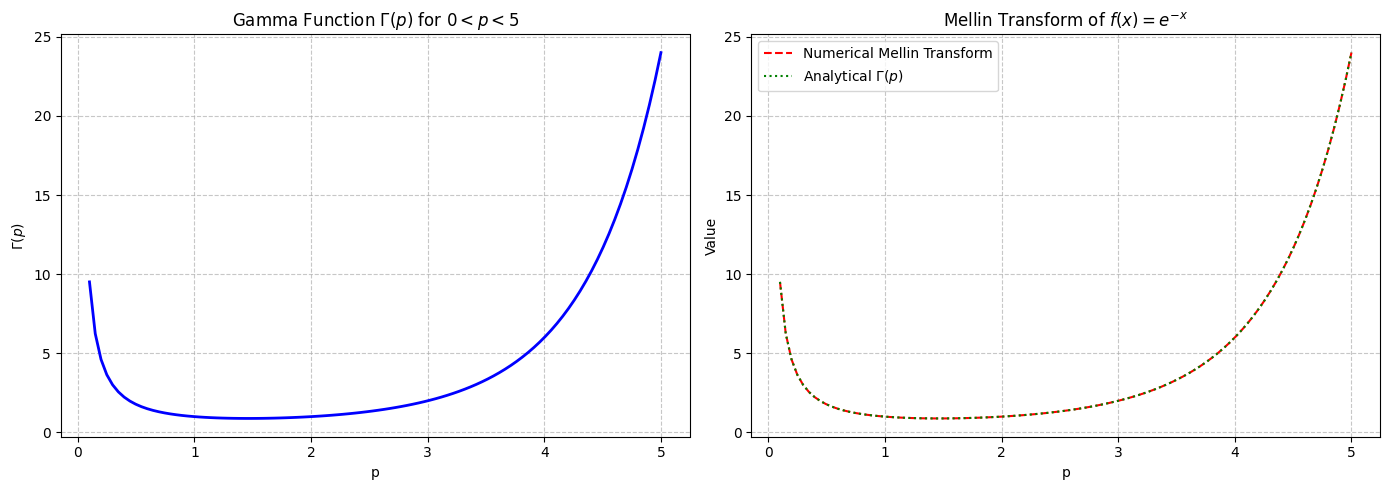
\includegraphics[width=0.8\textwidth]{Prooving Gamma function.png}
    \caption{Comparison of numerical Mellin Transform and analytical Gamma function for $f(x) = e^{-x}$.}
    \label{fig:gamma_vs_mellin}
\end{figure}

The plot demonstrates excellent agreement between the numerical and analytical results, confirming the relationship between the Mellin Transform of $f(x) = e^{-x}$ and the Gamma function.


\section{Verification for $f(x) = \frac{1}{x+1}$}

The function $f(x) = \frac{1}{x+1}$ serves as another example for exploring the Mellin Transform. The corresponding Mellin Transform is given by:
\begin{equation}
\int_{0}^{\infty} \frac{x^{p-1}}{x+1} \, dx = \frac{\pi}{\sin(\pi p)}.
\end{equation}
This integral identity highlights the connection between the Mellin Transform and trigonometric functions.

\subsection{Relationship with Gamma Functions}
The above identity can also be expressed using the Gamma function as:
\begin{equation}
\Gamma(p) \Gamma(1-p) = \frac{\pi}{\sin(\pi p)}.
\end{equation}
This relationship demonstrates the interplay between the Mellin Transform and the Gamma function, reinforcing its analytical significance.

\subsection{Python Implementation}
The following Python code was used to compute the Mellin Transform numerically, evaluate the Gamma product, and compare the results with the analytical solution:
\begin{verbatim}
import numpy as np
from scipy.special import gamma
import matplotlib.pyplot as plt
from scipy.integrate import quad

# Define the function
f = lambda x: 1 / (x + 1)

# Define Mellin Transform for f(x)
def mellin_transform(f, p):
    result, _ = quad(lambda x: x**(p-1) * f(x), 0, np.inf)
    return result

# Generate p values
p_values = np.linspace(0.1, 0.9, 100)

# Compute values
mt_values = [mellin_transform(f, p) for p in p_values]
gamma_product = [gamma(p) * gamma(1 - p) for p in p_values]
analytical = [np.pi / np.sin(np.pi * p) for p in p_values]

# Plot results
plt.figure(figsize=(10, 6))
plt.plot(p_values, mt_values, 'b-', label='Numerical Mellin Transform')
plt.plot(p_values, gamma_product, 'g--', label='Gamma Product')
plt.plot(p_values, analytical, 'r:', label='Analytical Solution')
plt.xlabel('p')
plt.ylabel('Value')
plt.title('Verification of Mellin Transform for $f(x) = \frac{1}{x+1}$')
plt.legend()
plt.grid(True)
plt.show()
\end{verbatim}

\subsection{Results and Visualization}
The results from the numerical computation, Gamma product, and analytical solution were plotted and compared. The plot below illustrates how closely these values align:

\begin{figure}[H]
    \centering
    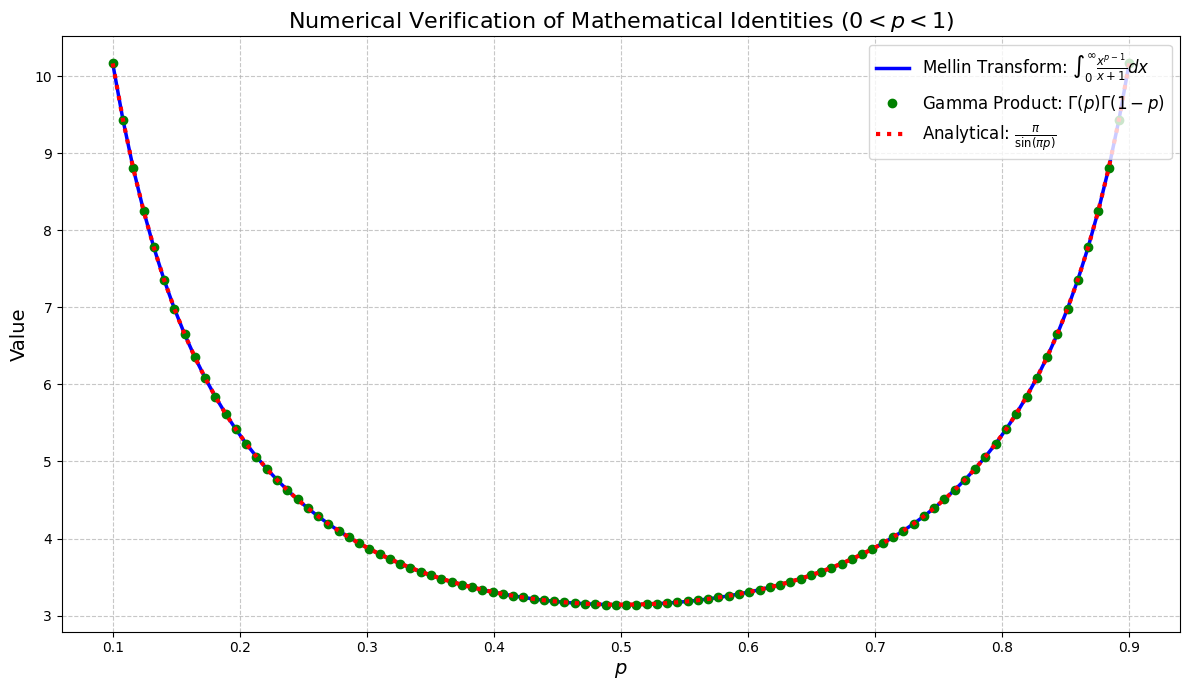
\includegraphics[width=0.8\textwidth]{Example.png}
    \caption{Numerical verification of mathematical identities for $f(x) = \frac{1}{x+1}$ ($0 < p < 1$).}
    \label{fig:mellin_identity}
\end{figure}

The alignment between the numerical results, Gamma product, and analytical solution validates the theoretical relationship. This example highlights the utility of the Mellin Transform in analyzing functions and verifying mathematical identities.


\section{Exploring Scaling and Shifting Properties}

The scaling and shifting properties of the Mellin Transform provide insights into the behavior of functions under transformations. These properties are defined and verified numerically below.

\subsection{Scaling Property}
The scaling property of the Mellin Transform states:
\begin{equation}
\mathcal{M}\{f(ax)\}(s) = a^{-s} \mathcal{M}\{f(x)\}(s),
\end{equation}
where $a > 0$. This property implies that scaling the argument of the function results in a multiplicative factor in the transform domain.

\subsection{Shifting Property}
The shifting property of the Mellin Transform is defined as:
\begin{equation}
\mathcal{M}\{x^a f(x)\}(s) = \mathcal{M}\{f(x)\}(s + a).
\end{equation}
This property describes how multiplying the function by a power of $x$ shifts the argument of the transform.

\subsection{Python Implementation}
The following Python code demonstrates the verification of both properties numerically:
\begin{verbatim}
import numpy as np
from scipy.integrate import quad
from scipy.special import gamma
import matplotlib.pyplot as plt

# Define Mellin transform function
def mellin_transform(f, p):
    result, _ = quad(lambda x: x**(p-1) * f(x), 0, np.inf)
    return result

# Define original and transformed functions
def f(x):
    return np.exp(-x)

def scaled_f(x, a):
    return f(a * x)

def shifted_f(x, a):
    return x**a * f(x)

# Parameters
a = 2
p_values = np.linspace(0.1, 5, 100)

# Compute values for scaling
scaling_numerical = [mellin_transform(lambda x: scaled_f(x, a), p) for p in p_values]
scaling_analytical = [a**-p * mellin_transform(f, p) for p in p_values]

# Compute values for shifting
shifting_numerical = [mellin_transform(lambda x: shifted_f(x, a), p) for p in p_values]
shifting_analytical = [mellin_transform(f, p + a) for p in p_values]

# Plot results
plt.figure(figsize=(12, 6))

# Scaling
plt.subplot(1, 2, 1)
plt.plot(p_values, scaling_numerical, 'bo', label='Numerical Scaling')
plt.plot(p_values, scaling_analytical, 'r--', label='Analytical Scaling')
plt.title(f'Scaling Property: $f(ax)$, $a = {a}$')
plt.xlabel('$s$')
plt.ylabel('Value')
plt.legend()

# Shifting
plt.subplot(1, 2, 2)
plt.plot(p_values, shifting_numerical, 'mo', label='Numerical Shifting')
plt.plot(p_values, shifting_analytical, 'g--', label='Analytical Shifting')
plt.title(f'Shifting Property: $x^a f(x)$, $a = {a}$')
plt.xlabel('$s$')
plt.ylabel('Value')
plt.legend()

plt.tight_layout()
plt.show()
\end{verbatim}

\subsection{Results and Visualization}
The results of the numerical verification for both properties are shown below:

\begin{figure}[H]
    \centering
    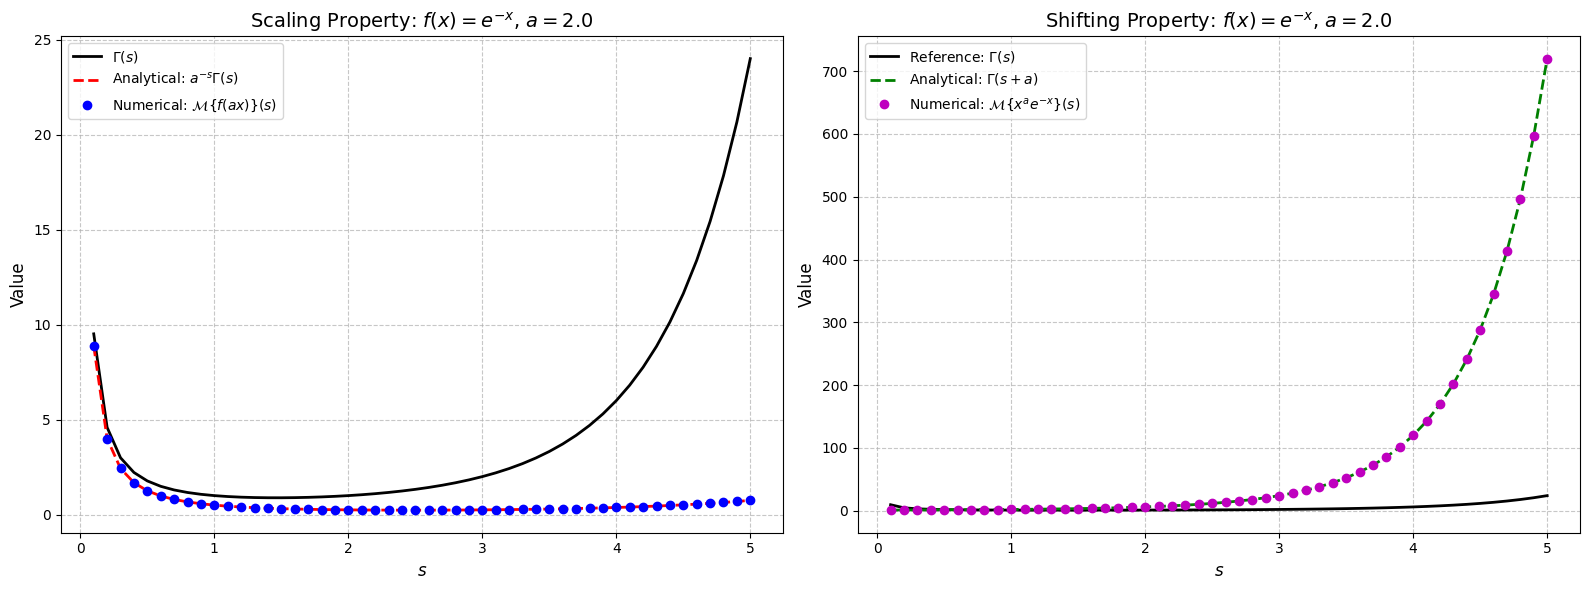
\includegraphics[width=0.8\textwidth]{Shifting and scaling.png}
    \caption{Numerical verification of scaling and shifting properties for $f(x) = e^{-x}$.}
    \label{fig:scaling_shifting}
\end{figure}

The plots confirm the agreement between the numerical results and the analytical expressions, validating the scaling and shifting properties of the Mellin Transform.


\section{Visualizing $\phi(r, \theta)$}

The function $\phi(r, \theta)$ is computed using a convolutional approach, which integrates over a function $f(\xi)$ weighted by another function $h(r/\xi, \theta)$. This is defined mathematically as:
\begin{equation}
\phi(r, \theta) = \int_{0}^{\infty} f(\xi) \frac{h(r/\xi, \theta)}{\xi} \, d\xi.
\end{equation}

\subsection{Role of $h(r, \theta)$ and $f(\xi)$}
- The function $h(r, \theta)$ acts as a kernel that modulates the input function $f(\xi)$ based on the parameters $r$ and $\theta$. It encodes information about the relationship between the scale $r$ and the angle $\theta$.
- The function $f(\xi)$ represents the input signal or data, which is convolved with the kernel $h(r, \theta)$ to produce the output $\phi(r, \theta)$.

\subsection{Python Implementation}
The following Python code demonstrates the computation of $\phi(r, \theta)$:
\begin{verbatim}
import numpy as np
from scipy.integrate import quad
import matplotlib.pyplot as plt

# Define h(r, theta)
def h_function(r, theta, alpha):
    n = np.pi / (2 * alpha)
    term1 = (r**n) * (1 + r**(2 * n)) * np.cos(n * theta)
    term2 = 1 + 2 * r**(2 * n) * np.cos(2 * n * theta) + r**(4 * n)
    return term1 / term2

# Define phi(r, theta)
def phi_function(r, theta, alpha, f):
    def integrand(xi):
        h_val = h_function(r / xi, theta, alpha)
        return f(xi) * h_val / xi
    return quad(integrand, 0, np.inf, limit=50)[0]

# Example f(xi)
def f_function(xi):
    return np.exp(-xi)

# Define range for theta and r
alpha = np.pi / 4
theta_values = np.linspace(-alpha, alpha, 50)
r_values = np.linspace(0.1, 5, 50)

# Compute phi(r, theta)
phi_values = np.zeros((len(r_values), len(theta_values)))
for i, r in enumerate(r_values):
    for j, theta in enumerate(theta_values):
        phi_values[i, j] = phi_function(r, theta, alpha, f_function)

# Plot results
R, THETA = np.meshgrid(r_values, theta_values)
plt.figure(figsize=(10, 6))
plt.contourf(R, THETA, phi_values.T, levels=50, cmap='viridis')
plt.colorbar(label='$\phi(r, \theta)$')
plt.title('$\phi(r, \theta)$ for $\theta \in [-\pi/4, \pi/4]$ and $r \in [0.1, 5]$')
plt.xlabel('r')
plt.ylabel('$\theta$')
plt.show()
\end{verbatim}

\subsection{Results and Visualization}
The contour plot of $\phi(r, \theta)$ is shown below:

\begin{figure}[H]
    \centering
    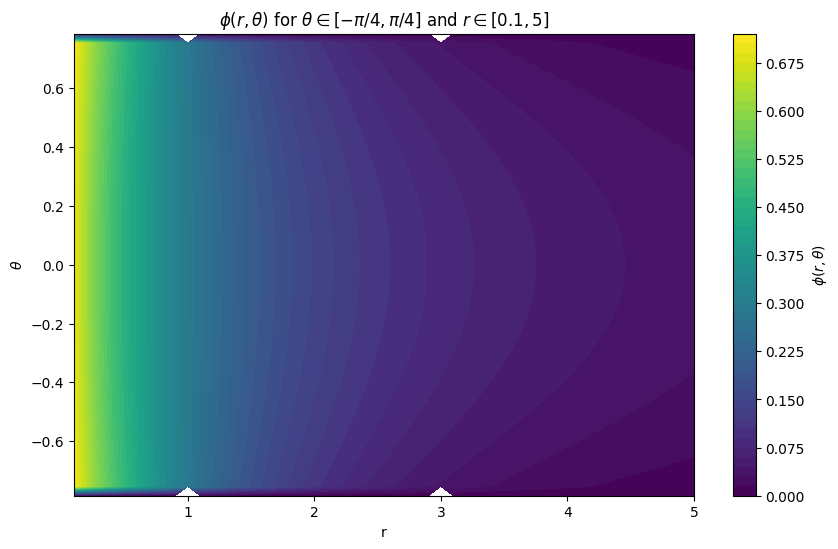
\includegraphics[width=0.8\textwidth]{Phi.png}
    \caption{Contour plot of $\phi(r, \theta)$ for $\theta \in [-\pi/4, \pi/4]$ and $r \in [0.1, 5]$.}
    \label{fig:phi_contour}
\end{figure}

This visualization demonstrates the variation of $\phi(r, \theta)$ with respect to the parameters $r$ and $\theta$. The results highlight the influence of the kernel $h(r, \theta)$ and the input function $f(\xi)$ on the output.

\section{Conclusion}
The Mellin Transform has been demonstrated as a powerful tool for analyzing functions, offering a unique way to study scale-invariant properties and multiplicative processes. This report verified key identities and properties such as scaling, shifting, and convolution-based calculations. The numerical implementations and their agreement with analytical results underscore the reliability of Python for mathematical analysis.

Potential extensions of this work include:
\begin{itemize}
    \item Exploring higher-dimensional Mellin Transforms to analyze multivariate functions.
    \item Applying the Mellin Transform in data science, such as feature extraction and signal decomposition.
    \item Investigating its role in solving advanced differential equations and integral equations.
\end{itemize}

\newpage

\clearpage

\section{References}

\begin{thebibliography}{99}
    \bibitem{Mellin} Debnath, Lokenath, and Dambaru Bhatta.\textit{l Transforms and Their Applications. 2nd ed.},CRC Press, 1995.
    \bibitem{Code} Github link,\textit{Application of Wavelet on EFIE} at \url{https://github.com/MohammadMahdiElyasi/Application-of-Wavelet-in-Elctromagnetic-Integral-Equation}.

\end{thebibliography}

\end{document}
